\section{Data files archived and stored}
\label{s:DataFilesArchived}
A naming convention for files and directories was used to separate each scan type from the other and each number of a scan.
In figure \ref{fig:FileNamingStructure} the structure of naming convention for files are shown.
The red color marks the task name, the blue marks the scan number, and the green contains the timestamp for the scan.
\begin{figure}[htbp]
\centerline{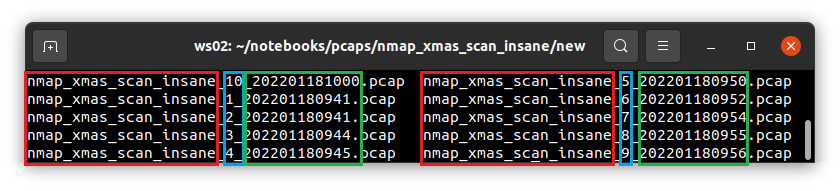
\includegraphics[scale=0.7]{images/misc/Files.png}}
\caption{File naming convention.}
\label{fig:FileNamingStructure}
\end{figure}

The directory structure shown in figure \ref{fig:DirNamingStructure} was created manually on the host running VMware Workstation, since the analysis using Jupyter was conducted on this host.
This was done mainly to separate each type of scan into respective subdirectories to prevent mixups of scan files and to keep a clean structure when conducting analysis.

\begin{figure}[htbp]
\centerline{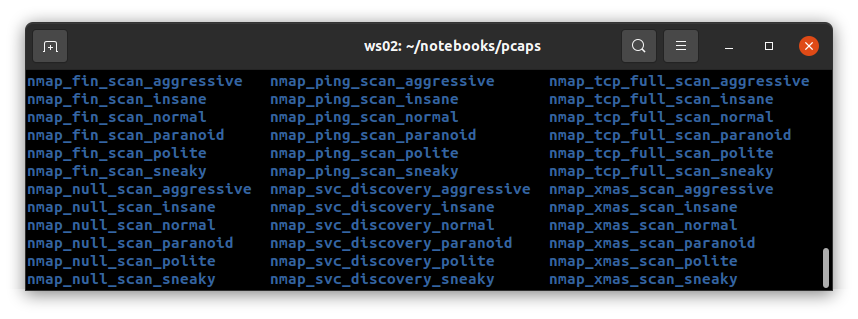
\includegraphics[scale=0.6]{images/misc/Directories.png}}
\caption{Directory naming convention.}
\label{fig:DirNamingStructure}
\end{figure}

The file listings on each of the worker hosts have no functionality to consider and sort the packet captures into respective subdirectories.
Each worker only saves the packet capture into their home directory with the naming convention shown in figure \ref{fig:FileNamingStructure}.

When the task list for all scans was completed, the \textsc{pcap retrieval}, further elaborated in section \ref{ss:PcapRetrieval} were executed manually.
All packet captures from the worker hosts were now transferred to the scanner host.
The packet captures retrieved could from here be retrieved through SSH from the host running VMware Workstation.
Before this retrieval can find place, the packet captures must be moved from the $root$ home to the $kali$ user's home directory, and the owner for directories and files must be changed to the $kali$ user before being able to retrieve these files. These steps are described in lines 2 and 3 in listing \ref{lst:FetchPcapFromScanner}.

\begin{listing}[!ht]
\caption{Limiting SSH to listen only to the management NIC}
\label{lst:FetchPcapFromScanner}
\begin{minted}[linenos]{Bash}
# The following commands must be executed as root on the scanner host
mv <directory where the packet captures are synched to> /home/kali/
chown -hR kali:kali /home/kali/<directory name mentioned above>

# If the VMware Workstation host is running Linux, the following commmand
# could be executed to retrieve all packet captures.
# This command must be executed at the VMware host machine
rsync -azvv -e ssh kali@<ip to scanner host>:<directory containing pcaps> \
<destination on scanner host>
# Example:
rsync -azvv -e ssh kali@192.168.2.230:pcap-results pcaps/
\end{minted}
\end{listing}

Within this research, the VMware host OS is Ubuntu Linux, which makes the transfer process of these files simple, and only the command in line 11 was executed to retrieve all packet captures.
Alternative tools for retrieving packet captures from the scanner host if the VMware host OS were Windows, WinSCP\footnote{https://winscp.net/} and Filezilla\footnote{https://filezilla-project.org/} are decent tools to use for this purpose. WinSCP has an easy GUI for transferring files, shown in figure \ref{fig:WinSCP}.

\begin{figure}[htbp]
\centerline{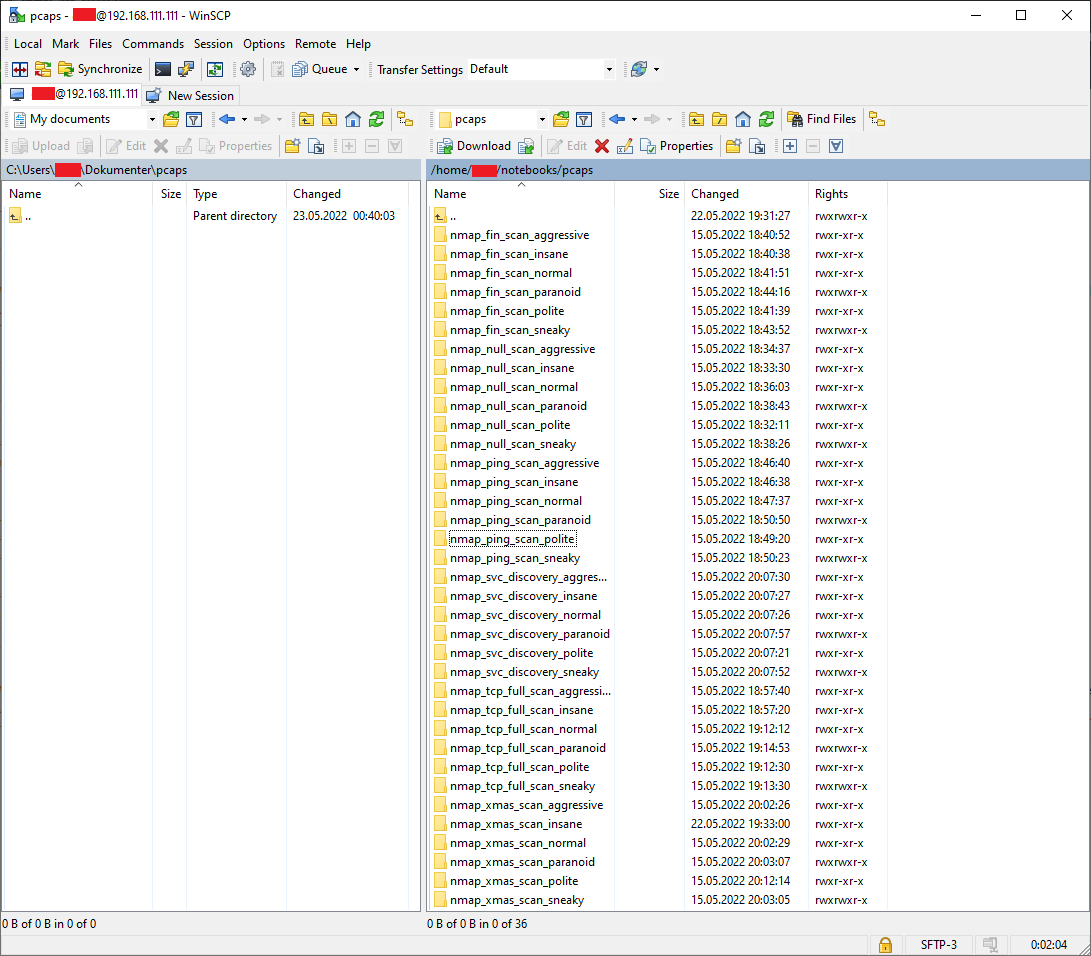
\includegraphics[scale=0.4]{images/misc/WinSCP.PNG}}
\caption{WinSCP GUI}
\label{fig:WinSCP}
\end{figure}